\section{Section overview}
\begin{itemize}
    \item Sequence: So far what we've learned has been sequential programming, a series of statements running sequentially, our code can't make decisions.
    \item Selection structures: allow us to make decisions based on certain conditions being true or false.
    \item Iteration: looping or repeating.
\end{itemize}

With sequence, selection and iteration we can implement any algorithm.

\subsection{Selection: Decision}
\begin{itemize}
    \item \mintinline{cpp}{if} statement.
    \item \mintinline{cpp}{if else} statement.
    \item Nested \mintinline{cpp}{if} statements.
    \item \mintinline{cpp}{switch} statement.
    \item Conditional operator \mintinline{cpp}{?:;}
\end{itemize}

\subsection{Iteration: Looping}
\begin{itemize}
    \item \mintinline{cpp}{for} loop.
    \item Range-Based \mintinline{cpp}{for} loop.
    \item \mintinline{cpp}{while} loop.
    \item \mintinline{cpp}{continue} and \mintinline{cpp}{break}.
    \item Infinite loops.
    \item Nested loops.
\end{itemize}


%----------------------------------------------------------------------------------------
\section{If statement}
\begin{itemize}
    \item Syntax is: \verb|if (expr) { statement; }|.
    \item The control expression must evaluate to a boolean true or false value.
    \item If the expression is true then execute the statement.
    \item If the expression is false then skip the statement.
    \item As a recommendation we always indent the code inside the if statement.
\end{itemize}

\subsection{Examples of single if statements}
For single if statements you do not need to enclose the statements in curly braces.
\begin{figure}[H]
    \centering
    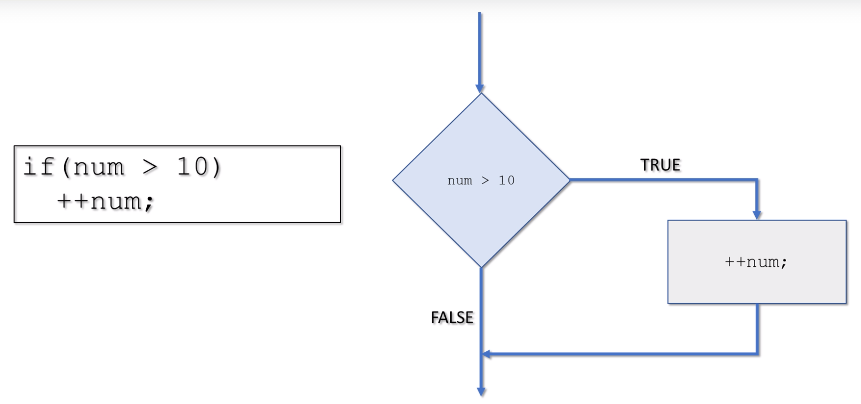
\includegraphics[width=0.4\textwidth]{./figs/single_if}
\end{figure}
\begin{minted}[autogobble]{cpp}
    if (selection == 'A')
        cout << "You selected A";
    if (num > 10)
        cout << "num is grater than 10";
    if (health < 100 && player_healed)
        health = 100;
\end{minted}

\subsection{Block if statements}
\begin{itemize}
    \item A block of code we have already seen in the main function.
    \item Create a block of code by including more than one statement in code block and adding \{\}.
    \item Blocks can also contain variable declarations.
    \item These variables are visible only within the block (local scope).
\end{itemize}
\begin{figure}[H]
    \centering
    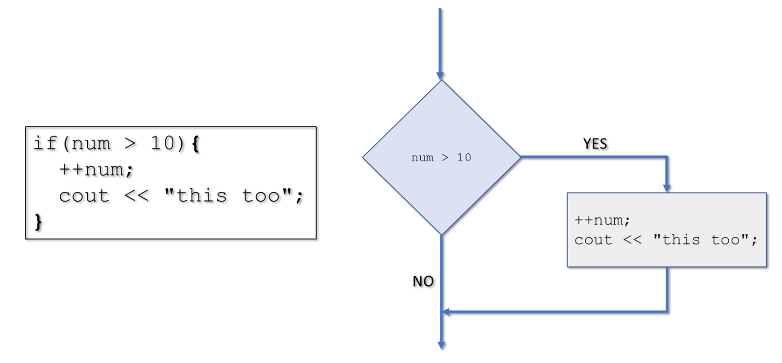
\includegraphics[width=0.4\textwidth]{./figs/multi_if}
\end{figure}

\subsection{Example of block ifs}
\begin{minted}[autogobble]{cpp}
    #include <iostream>
    using namespace std;
    int main() {
        int num {0};
        const int min {10}, max {100};
        cout << "Enter a number between " << min << " and " << max << ": ";
        cin >> num;
        if (num >= min) {
            cout << "\n================if statment 1===================" << endl;
            cout << num << " is grater than " << min << endl;
            int diff {num - min};
            cout << num << " is " << diff << " greater than " << min << endl;
        }

        if (num <= max) {
            cout << "\n================if statment 2===================" << endl;
            cout << num << " is less than or equal to " << max << endl;
            int diff {max - num};
            cout << num << " is " << diff << " less than " << max << endl;
        }

        if (num >= min && num <= max) {
            cout << "\n================if statment 3===================" << endl;
            cout << num << " is in range " << endl;
            cout << "This means statement 1 and 2 must also display!" << endl;
        }
        if (num == min || num == max) {
            cout << "\n================if statment 4===================" << endl;
            cout << num << " is in boundaries " << endl;
            cout << "This means statement 1, 2 and 3 must also display!" << endl;
        }
        return 0;
    }
    /* OUTPUT:
    Enter a number between 10 and 100: 100

    ================if statment 1===================
    100 is grater than 10
    100 is 90 greater than 10

    ================if statment 2===================
    100 is less than or equal to 100
    100 is 0 less than 100

    ================if statment 3===================
    100 is in range
    This means statement 1 and 2 must also display!

    ================if statment 4===================
    100 is in boundaries
    This means statement 1, 2 and 3 must also display!

    */
\end{minted}


%----------------------------------------------------------------------------------------
\section{If else statement}
\begin{itemize}
    \item Syntax:
        \begin{minted}[autogobble]{cpp}
            if (expr)
                statement;
            else
                statement2;
        \end{minted}
    \item If the expression is true then execute statement1.
    \item If the expression is false then execute statement2.
    \item Never forget the indentation.
\end{itemize}
\begin{figure}[H]
    \centering
    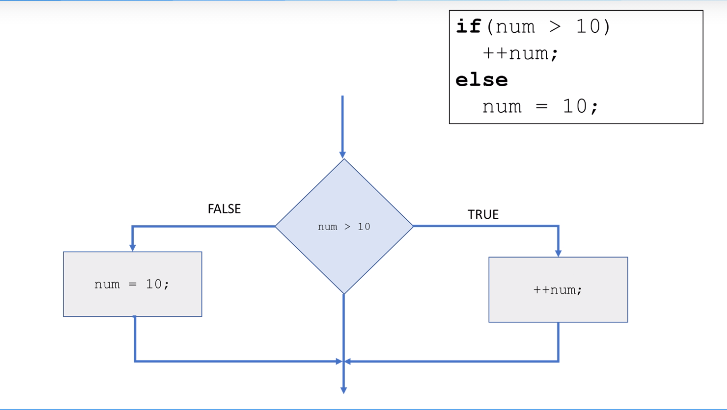
\includegraphics[width=0.4\textwidth]{./figs/ifelse}
\end{figure}

\subsection{Example of single if else statements}
\begin{minted}[autogobble]{cpp}
    if (num > 10)
        cout << "num is greater than 10";
    else 
        cout << "num is NOT greater than 10";
    
    if (health < 100 && heal_player) 
        health = 100;
    else 
        ++health;
\end{minted}


\subsection{If else block}
\begin{figure}[H]
    \centering
    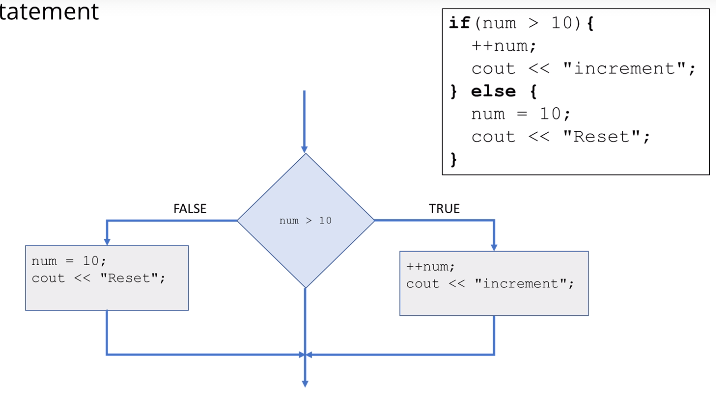
\includegraphics[width=0.4\textwidth]{./figs/multiifelse.png}
\end{figure}


\subsection{If else if construct}
\begin{itemize}
    \item Sometimes we need to check multiple conditions not just weather the expression is true but other characteristics, for this we use an if else if construct.
\end{itemize}
\begin{minted}[autogobble]{cpp}
    if (score > 90)
        cout << "A";
    else if (score > 80)
        cout << "B";
    else if (score > 70)
        cout << "C";
    else if (score > 60)
        cout << "D";
    else
        cout << "F";
    cout << "Done";
\end{minted}

\subsection{Example}
\begin{minted}[autogobble]{cpp}
    #include <iostream>
    using namespace std;
    int main() {
        int num{};
        const int target {10};
        cout << "Enter a number and I'll compare it to " << target << ": ";
        cin >> num;

        if (num >= target) {
            cout << "\n==========================" << endl;
            cout << num << " is greater than or equal to " << target << endl;
            int diff {num - target};
            cout << num << " is " << diff << " greater than " << target << endl;
        } else {
            cout << "\n==========================" << endl;
            cout << num << " is less than " << target << endl;
            int diff {target - num};
            cout << num << " is " << diff << " less than " << target << endl;
        }
        cout << endl;
        return 0;
    }
    /* OUTPUT:
    Enter a number and I'll compare it to 10: -10

    ==========================
    -10 is less than 10
    -10 is 20 less than 10

    */
\end{minted}


%----------------------------------------------------------------------------------------
\section{Nested if statement}
\begin{itemize}
    \item You can nest if statements within other if statements.
        \begin{minted}[autogobble]{cpp}
            if (expr1) 
                if (expr2) 
                    statement1;
                else 
                    statement2;
        \end{minted}
    
    \item If the expression is true then execute statement1.
    \item If the expression is false then execute statement2.
    \item Many times we need more logic to the if statement.
    \item In the above example the if statement expects one statement without the curly braces, however the if statement is a one compound statement and that is why the above code doesn't need curly braces.
    \item Notice, how does the computer know if the else statement belongs to the closest or farthest if? In C++ each else belogs to the closest if, so in the above example it belongs to the if holding the expr2.
    \item Remember to indent.
\end{itemize}

\subsection{Example}
\begin{itemize}
    \item Example of scores:
        \begin{minted}[autogobble]{cpp}
            if (score > 90) 
                if (score > 95)
                    cout << "A+";
                else 
                    cout << "A";
            cout << "Sorry, No A";
        \end{minted}
        \begin{figure}[H]
            \centering
            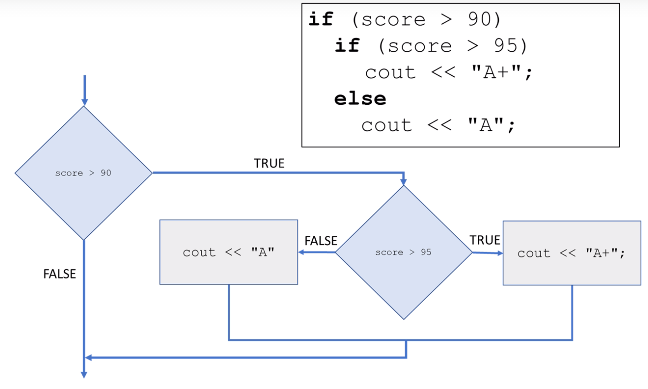
\includegraphics[width=0.4\textwidth]{./figs/exnestedif.png}
        \end{figure}
    
    \item Example:
        \begin{minted}[autogobble]{cpp}
            if (score_frank != score_bill) {
                if (score_frank > score_bill) {
                    cout << "Frank wins" << endl;
                } else {
                    cout << "Bill wins" << endl;
                }
            } else {
                cout << "Looks like a tie!" << endl;
            }
        \end{minted}
    
    \item Example of nested latter:
        \begin{minted}[autogobble]{cpp}
            #include <iostream>
            using namespace std;
            int main() {
                int score {};
                cout << "Enter your score in the exam (0-100): ";
                cin >> score;
                char letter_grade {};

                if (score >= 0 && score <= 100) {
                    if (score >= 90)
                        letter_grade = 'A';
                    else if (score >= 80)
                        letter_grade = 'B';
                    else if (score >= 70)
                        letter_grade = 'C';
                    else if (score >= 60)
                        letter_grade = 'D';
                    else
                        letter_grade = 'F';
                    cout << "Your grade is: " << letter_grade << endl;
                    if (letter_grade == 'F') 
                        cout << "Bad grade." << endl;
                    else 
                        cout << "Congrats." << endl;
                } else {
                    cout << "Sorry, " << score << "is not in range." << endl;
                }
                return 0;
            }
            /* OUTPUT:
            Enter your score in the exam (0-100): 90
            Your grade is: A
            Congrats.

            */
        \end{minted}
\end{itemize}


%----------------------------------------------------------------------------------------
\section{Switch-case statement}
\begin{itemize}
    \item There are some applications where you need to execute certain blocks of code depending on the value of a constant, for this you can use the \mintinline{cpp}{switch} statement.
        \begin{minted}[autogobble]{cpp}
            switch (integer_control_expr) {
                case expression_1: statement_1; break;
                case expression_2: statement_2; break;
                case expression_3: statement_3; break;
                case expression_4: statement_4; break;
                ...;
                default: statement_default; break;
            }
        \end{minted}
    \item Syntax: The switch keyword is followed by the control expression in parentheses. This control expression must evaluate to an integer type or an enumeration type. Then you have a series of case statements, the value of the control expression will be compared to the values contained in each case, these also need to be constants or literals pertaining to an enumeration or integral type. If no values match the switch will execute the default, this is like the else. The break statement in C++ are optional but best practice is to include them unless you have a very good reason not to. A break statement is not needed in the default case.
    \item If one case is followed by another such as: the switch will act as a logical or.
        \begin{minted}[autogobble]{cpp}
            case '3':
            case '4': cout << "3 or 4 selected";
        \end{minted}
        It is the same as saying:
        \begin{minted}[autogobble]{cpp}
            if ('3' || '4') 
                cout << "3 or 4 selected";
        \end{minted}
    
    \item Once the switch has hit a match, no further cases will be checked.
\end{itemize}

\subsection{Example}
\begin{itemize}
    \item Suppose \mintinline{cpp}{selection} is an character initialized to the character 2.
        \begin{minted}[autogobble]{cpp}
            switch (selection) {
                case '1': cout << "1 selected"; // compare selection to 1, not true.
                        break;
                case '2': cout << "2 selected"; // compare selection to 2, is true, execute the code from the colon to the break.
                        break;
                case '3': cout << "3 selected";
                        break;
                case '4': cout << "4 selected";
                        break;
                default: cout << "1,2,3,4 NOT selected";
            }
        \end{minted}
    
    \item Example of fall-through:
        \begin{minted}[autogobble]{cpp}
            #include <iostream>
            using namespace std;
            int main() {
                char selection {'2'};
                switch (selection) {
                    case '1': cout << "1 selected\n";
                            break;
                    case '2': cout << "2 selected\n"; // this case evaluates 2 or 3 or 4 or 5.
                    case '3': cout << "3 selected\n";
                    case '4': cout << "4 selected\n";
                    case '5': cout << "5 selected\n";
                            break;
                    case '6': cout << "4 selected\n";
                            break;
                    default: cout << "1,2,3,4 NOT selected\n";
                }
                return 0;
            }
            /* OUTPUT:
            2 selected
            3 selected
            4 selected
            5 selected

            */
        \end{minted}
    
    \item The switch statement is commonly used with enumeration, meaning the \mintinline{cpp}{enum}, for example: 
        \begin{minted}[autogobble]{cpp}
            #include <iostream>
            using namespace std;
            int main() {
                enum Color {
                    red, green, blue
                };
                Color screen_color {green};
                switch (screen_color) {
                    case red: cout << "red"; break;
                    case green: cout << "green"; break;
                    case blue: cout << "blue"; break;
                    default: cout << "should never execute";
                }
                return 0;
            }
            /* OUTPUT:
            green
            */
        \end{minted}
\end{itemize}

\subsection{Review}
\begin{itemize}
    \item The control expression must evaluate to an integer type.
    \item The case expressions must be constant expressions that evaluate to integer or integers literals. They must be constants or literals, no variables.
    \item Once a match occurs all the code in the case statement is executed until a break is reached, then the switch terminates.
    \item Best practice is to provide break statement for each case.
    \item Best practice is also to provide \mintinline{cpp}{default} case, this is optional but should be handled in case it does get executed.
\end{itemize}

\subsection{Example}
\begin{itemize}
    \item Switch with characters: 
        \begin{minted}[autogobble]{cpp}
            #include <iostream>
            using namespace std;
            int main() {
                char letter_grade{};
                cout << "Enter the letter grade you expect on the exam: ";
                cin >> letter_grade;
                switch (letter_grade) {
                case 'a':
                case 'A':
                    cout << "90 or above." << endl;
                    break;
                case 'b':
                case 'B':
                    cout << "80-89" << endl;
                    break;
                case 'c':
                case 'C':
                    cout << "70-79" << endl;
                    break;
                case 'd':
                case 'D':
                    cout << "60-69" << endl;
                    break;
                case 'f':
                case 'F': {
                    char confirm{};
                    cout << "Are you sure (Y/N)?";
                    cin >> confirm;
                    if (confirm == 'y' || confirm == 'Y') {
                        cout << "0-60" << endl;
                    } else {
                        cout << "Illegal choice." << endl;
                    }
                    break;
                }
                default:
                    cout << "Invalid input." << endl;
                    break;
                }
                return 0;
            }
            /* OUTPUT:
            Enter the letter grade you expect on the exam: f
            Are you sure (Y/N)?y
            0-60

            */
        \end{minted}
    
    \item Switch with enumeration (\mintinline{cpp}{enum}):
        \begin{minted}[autogobble]{cpp}
            #include <iostream>
            using namespace std;
            int main() {
                enum Direction {
                    left, right, up, down
                };
                Direction heading {left};

                switch (heading) {
                    // some compilers won't let you compile if you don't handle every case. So it would not compile if we forget to  handle the 'right' case for example.
                    case left:
                        cout << "Going left" << endl;
                        break;
                    case right:
                        cout << "Going right" << endl;
                        break;
                    case up:
                        cout << "Going up" << endl;
                        break;
                    case down:
                        cout << "Going down" << endl;
                        break;
                    default: 
                        cout << "OK" << endl;
                }
                return 0;
            }
            /* OUTPUT:
            Going left
            */
        \end{minted}
\end{itemize}


%----------------------------------------------------------------------------------------
\section{Conditional operator}
\begin{itemize}
    \item Syntax is: \verb|(cond_expr) ? expr1 : expr2;|
    \item This is frequently called the ternary operator.
    \item \verb|cond_expr| evaluates to a boolean expression.
        \begin{itemize}
            \item If \verb|cond_expr| is true the value of \verb|expr1| is returned.
            \item If \verb|cond_expr| is false the value of \verb|expr2| is returned.
        \end{itemize}
    \item Similar to an if-else construct in a single expression.
    \item Ternary operator.
    \item Very useful when used inline.
    \item Very easy to abuse! Best practice is to never nest a conditional operator within another one, this causes the code to become unreadable and difficult to manage.
\end{itemize}

\subsection{Example}
\begin{itemize}
    \item Example:
        \begin{minted}[autogobble]{cpp}
            #include <iostream>
            using namespace std;
            int main() {
                int a {10}, b {20};
                int score {92};
                int result {};
                result = (a > b) ? a : b; // false.
                cout << result << endl;
                result = (a < b) ? (a - b) : (a-b); // true.
                cout << result << endl;
                result = (b != 0) ? (a / b) : 0; // false.
                cout << result << endl;
                cout << ((score > 90)? "Excelent":"Good"); // true.
                return 0;
            }
            /* OUTPUT:
            20
            -10
            0
            Excelent
            */
        \end{minted}
    
    \item You can use conditional operators to write ifs in one single line:
        \begin{minted}[autogobble]{cpp}
            #include <iostream>
            using namespace std;
            int main() {
                int num {};
                cout << "Enter an int: ";
                cin >> num;
                // usually written with ifs: 
                if (num % 2 == 0) 
                    cout << num << " is even." << endl;
                else 
                    cout << num << " is odd." << endl,
                cout << endl;

                // you could do it with the conditional operator:
                cout << num << " is" << ((num % 2 == 0) ? " even." : " odd.") << endl;

                return 0;
            }
            /* OUTPUT:
            Enter an int: 6
            6 is even.
            6 is even.

            */
        \end{minted}
    
    \item Another example: 
        \begin{minted}[autogobble]{cpp}
            #include <iostream>
            using namespace std;
            int main() {
                int num1 {}, num2 {};
                cout << "Enter two integers separated by a space: ";
                cin >> num1 >> num2;
                if (num1 != num2) {
                    cout << "Largest: " << ((num1 > num2)?num1:num2) << endl;
                } else {
                    cout << "The numbers are the same." << endl;
                }
                return 0;
            }
            /* OUTPUT:
            Enter two integers separated by a space: 10 11
            Largest: 11

            */
        \end{minted}
\end{itemize}


%----------------------------------------------------------------------------------------
\section{Looping}
\begin{itemize}
    \item Looping is also called iteration and is the third basic building block of programming. 
        \begin{itemize}
            \item Sequence, selection, iteration. Remember with these building blocks you can implement any algorithm.
        \end{itemize}
    
    \item Iteration or repetition.
    \item Allows the execution of a statement or block of statements repeatedly.
    \item Loops are made up of a loop condition and the body which contains the statements to repeat.
\end{itemize}

\subsection{Use cases of looping}
Execute a loop: 
\begin{itemize}
    \item A specific number of times, such as the user enters the number of times.
    \item For each element in a collection of elements.
    \item While specific condition(s) remains true.
    \item Until a specific condition becomes false.
    \item Until we reach the end of some input stream.
    \item Forever (infinite loops) (for example operating systems).
    \item Many, many more use cases.
\end{itemize}

\subsection{C++ looping constructs}
\begin{itemize}
    \item \mintinline{cpp}{for} loop:
        \begin{itemize}
            \item Iterate specific number of times.
        \end{itemize}
    
    \item Range-based for loop:
        \begin{itemize}
            \item One iteration for each element in a range or collection.
            \item Used with arrays and vectors for example.
        \end{itemize}
    
    \item \mintinline{cpp}{while} loop:
        \begin{itemize}
            \item Iterate while condition remains true.
            \item Stop when the condition becomes false.
            \item Check the condition at the beginning of every iteration.
        \end{itemize}
    
    \item \mintinline{cpp}{do while} loop:
        \begin{itemize}
            \item Iterate while a condition remains true.
            \item Stop when the condition is false.
            \item Check the condition at the end of every iteration.
            \item The same as the while loop only difference is that the do while checks the condition after each iteration, the while loop checks conditions before each iteration.
        \end{itemize}
\end{itemize}


%----------------------------------------------------------------------------------------
\section{\mintinline{cpp}{for} loop}
\begin{itemize}
    \item You can omit the curly braces if only one statement will be executed, if two or more are executed that will need to be enclosed in a block of code.
        \begin{minted}[autogobble]{cpp}
            for (initalization; condition; increment)
                statement;
            for (initalization; condition; increment) {
                statement1;
                statement2;
                statementn;
            }
        \end{minted}
    
    \item The initialization is executed exactly once. Then the condition is checked, if its true it will execute the block of code and then the increment will take place, when the condition evaluates to false the loop terminates.
\end{itemize}

\subsection{Examples}
\begin{itemize}
    \item Count from one to five:
        \begin{minted}[autogobble]{cpp}
            #include <iostream>
        using namespace std;
        int main() {
            int i {0};
            for (i = 1; i <= 5; ++i) {
                cout << i << endl;
            }

            return 0;
        }
        /* OUTPUT:
        1
        2
        3
        4
        5
        */
        \end{minted}
    
    \item You can declare the conter variable (if you must use one) and initialize all inside the for loop, the advantage to this is that you don't need to declare it outside (like the previous example), however that variable will remain only within the score of the for loop, you cannot use it else where.
        \begin{minted}[autogobble]{cpp}
            #include <iostream>
            using namespace std;
            int main() {
                for (int i {1}; i <= 5; ++i) {
                    cout << i << endl;
                }
                for (int i = 1; i <= 5; ++i) {
                    cout << i << endl;
                }
                cout << i << endl; // compiler error, i was not declared in this scope.
                return 0;
            }
        \end{minted}
        Correction: 
        \begin{minted}[autogobble]{cpp}
            #include <iostream>
            using namespace std;
            int main() {
                for (int i {1}; i <= 5; ++i) {
                    cout << i << endl;
                }
                for (int i = 1; i <= 5; ++i) {
                    cout << i << endl;
                }
                return 0;
            }
            /* OUTPUT:
            1
            2
            3
            4
            5
            1
            2
            3
            4
            5
            */
        \end{minted}
    
    \item Display even numbers from one to ten:
        \begin{minted}[autogobble]{cpp}
            #include <iostream>
            using namespace std;
            int main() {
                for (int i {1}; i <= 10; ++i) {
                    if (i % 2 == 0) {
                        cout << i << endl;
                    }
                }
                return 0;
            }
            /* OUTPUT:
            2
            4
            6
            8
            10
            */
        \end{minted}
    
    \item Use for loops to iterate an array: 
        \begin{minted}[autogobble]{cpp}
            #include <iostream>
            using namespace std;
            int main() {
                int scores[] {100,90,87};
                for (int i {0}; i < 3; ++i) {
                    cout << scores[i] << endl;
                }
                return 0;
            }
            /* OUTPUT:
            100
            90
            87
            */
        \end{minted}
        \begin{itemize}
            \item Very careful with array out of bounds errors.
        \end{itemize}
    
    \item You can initialize many variables using the comma operator:
        \begin{minted}[autogobble]{cpp}
            #include <iostream>
            using namespace std;
            int main() {
                for (int i {1}, j {5}; i <= 5; ++i, ++j) {
                    cout << i << " * " << j << " : " << (i * j) << endl;
                }
                return 0;
            }
            /* OUTPUT:
            1 * 5 : 5
            2 * 6 : 12
            3 * 7 : 21
            4 * 8 : 32
            5 * 9 : 45
            */
        \end{minted}
        \begin{itemize}
            \item Note that the associativity is right to left, and the result of the comma operator is the left most expression.
            \item In this case we just use them to initialize two variables and then to increment those two variables.
        \end{itemize}
\end{itemize}

\subsection{Other details}
\begin{itemize}
    \item The basic for loop is very clear and concise.
    \item Since the for loop's expressions are all optional, it is possible to have:
        \begin{itemize}
            \item No initialization, No condition, and No increment.
            \item This creates an infinite loop, and as we will see later on is the same as using the while loop with the condition being just true always.
            \item You can also use doubles and other types as counters.
            \item Best practice is to never include any expressions too complicated to document, if the expressions are too complicated consider using another looping construct.
        \end{itemize}
        \begin{minted}[autogobble]{cpp}
            for (;;) {
                cout << "Endless loop" << endl;
            }
        \end{minted}
\end{itemize}

\subsection{Examples}
\begin{itemize}
    \item Count from one to ten:
        \begin{minted}[autogobble]{cpp}
            #include <iostream>
            using namespace std;
            int main() {
                for (int i {1}; i <= 10; ++i) {
                    cout << i << endl;
                }
                return 0;
            }
            /* OUTPUT:
            1
            2
            3
            4
            5
            6
            7
            8
            9
            10
            
            */
        \end{minted}
    
    \item Count from one to ten every two:
        \begin{minted}[autogobble]{cpp}
            #include <iostream>
            using namespace std;
            int main() {
                for (int i {1}; i <= 10; i += 2) {
                    cout << i << endl;
                }
                return 0;
            }
            /* OUTPUT:
            1
            3
            5
            7
            9

            */
        \end{minted}
    
    \item For decrementing:
        \begin{minted}[autogobble]{cpp}
            #include <iostream>
            using namespace std;
            int main() {
                for (int i {10}; i > 0; --i) {
                    cout << i << endl;
                }
                return 0;
            }
            /* OUTPUT:
            10
            9
            8
            7
            6
            5
            4
            3
            2
            1

            */
        \end{minted}
    
    \item Iterating a vector:
        \begin{minted}[autogobble]{cpp}
            #include <iostream>
            #include <vector>
            using namespace std;
            int main() {
                vector<int> nums {10,20,30,40,50};
                for (unsigned i{0}; i < nums.size(); ++i) {
                    cout << nums[i] << endl;
                }
                return 0;
            }
            /* OUTPUT:
            10
            20
            30
            40
            50

            */
        \end{minted}
\end{itemize}


%----------------------------------------------------------------------------------------
\section{Range based for loop}
\begin{itemize}
    \item The idea with the range based for loop is to loop through a collection of elements and be able to easily access each element, without having to worry about the length of the collection or incrementing or decrementing looping variables or subscripting indexes. 
    \item The syntax is: 
        \begin{verbatim}
            for (var_type var_name : collection_name) 
                statement1; // can use var_name.
                for (var_type var_name : collection_name) {
                    statements; // can use var_name.
                }
        \end{verbatim}
    \item \verb|var_type| will be bound to each element of the collection so it should be of the same type the collection of elements.
    \item Now when we access each variable name in the loop it will have a specific element in the collection.
    \item For example:
        \begin{minted}[autogobble]{cpp}
            #include <iostream>
            using namespace std;
            int main() {
                int scores[] {100,90,97};
                for (int score : scores) {
                    cout << score << endl;
                }
                return 0;
            }
            /* OUTPUT:
            100
            90
            97

            */
        \end{minted}
    
    \item Instead of providing the \verb|var_type| you can use the \mintinline{cpp}{auto} keyword, this allows the C++ compiler to deduce the type itself.
        \begin{minted}[autogobble]{cpp}
            #include <iostream>
            using namespace std;
            int main() {
                int scores[] {100,90,97};
                for (auto score : scores) {
                    cout << score << endl;
                }
                return 0;
            }
            /* OUTPUT:
            100
            90
            97

            */
        \end{minted}
\end{itemize}

\subsection{Examples}
\begin{itemize}
    \item Vector example:
        \begin{minted}[autogobble]{cpp}
            #include <iostream>
            #include <vector>
            using namespace std;
            int main() {
                vector<double> temps {87.2, 77.1, 80.0, 72.5};
                double average_temp {};
                double running_sum {};
                for (auto temp : temps) {
                    running_sum += temp;
                }
                average_temp = running_sum / temps.size();
                cout << average_temp << endl;
                return 0;
            }
            /* OUTPUT:
            79.2
            */
        \end{minted}
    
    \item Intializer list:
        \begin{minted}[autogobble]{cpp}
            #include <iostream>
            using namespace std;
            int main() {
                double average_temp {};
                double running_sum {};
                int size {};
                for (auto temp : {60.2, 80.1, 90.0, 78.2}) {
                    running_sum += temp; size++;
                }
                average_temp = running_sum / size;
                cout << average_temp << endl;
                return 0;
            }
            /* OUTPUT:
            77.125
            */
        \end{minted}
    
    \item Looping a string:
        \begin{minted}[autogobble]{cpp}
            #include <iostream>
            using namespace std;
            int main() {
                for (auto c: "C++") {
                    cout << c << endl;
                }
                return 0;
            }
            /* OUTPUT:
            C
            +
            +

            */
        \end{minted}
\end{itemize}


%----------------------------------------------------------------------------------------
\section{While}
\begin{itemize}
    \item The while loop is an example of a pre-test loop because the expression is evaluated before executing the code. 
    \item If the expression evaluates to true the code is executed, else it is not executed.
    \item Syntax is: 
        \begin{verbatim}
            while (expression) 
                statement;
            while (expression) {
                statement (s);
            }
        \end{verbatim}
    \item The \verb|expression| has to evaluate to a boolean value. Followed by the statement or the block of statements.
\end{itemize}

\subsection{Example}
\begin{itemize}
    \item Counting from 1-5.
        \begin{minted}[autogobble]{cpp}
            #include <iostream>
            using namespace std;
            int main() {
                int i {1};
                while (i <= 5) {
                    cout << i << endl;
                    ++i; // increment
                }
                return 0;
            }
            /* OUTPUT:
            1
            2
            3
            4
            5

            */
        \end{minted}
    
    \item Even numbers between 1 and 10.
        \begin{minted}[autogobble]{cpp}
            #include <iostream>
            using namespace std;
            int main() {
                int i {1};
                while (i <= 10) {
                    if (i % 2 == 0) 
                        cout << i << endl;
                    ++i;
                }
                return 0;
            }
            /* OUTPUT:
            2
            4
            6
            8
            10

            */
        \end{minted}
    
    \item Array example:
        \begin{minted}[autogobble]{cpp}
            #include <iostream>
            using namespace std;
            int main() {
                int scores[] {100,90,87};
                int i {0};
                while (i < 3) {
                    cout << scores[i] << endl;
                    ++i;
                }
                return 0;
            }
            /* OUTPUT:
            100
            90
            87

            */
        \end{minted}
    
    \item Input validation:
        \begin{minted}[autogobble]{cpp}
            #include <iostream>
            using namespace std;
            int main() {
                int number {};
                cout << "Enter an integer less than 100: ";
                cin >> number;
                while (number < 100) {
                    cout << "Enter an integer less than 100: ";
                    cin >> number;
                }
                cout << "Thanks" << endl;
                return 0;
            }
            /* OUTPUT:
            Enter an integer less than 100: 100
            Enter an integer less than 100: 99
            Thanks

            */
        \end{minted}
\end{itemize}


%----------------------------------------------------------------------------------------
\section{do-while loop}
\begin{itemize}
    \item Syntax is: 
        \begin{verbatim}
            do {
                statements;
            } while (expression);
        \end{verbatim}
    \item The do-while loop is a post-test loop, because the expression is tested at the end of each iteration.
    \item This means that the loop body is garanteed to be executed at least once.
\end{itemize}

\subsection{Examples}
\begin{itemize}
    \item Input validation:
        \begin{itemize}
            \item In the below code, notice that variable declarations cannot be done inside the do-while code body, if you do this you will get a compiler error. 
            \item You cannot declare variables that are involved in the expression inside the code body.
        \end{itemize}
        \begin{minted}[autogobble]{cpp}
            #include <iostream>
            using namespace std;
            int main() {
                int number {};
                do {
                    cout << "Enter an integer between 1 and 5: ";
                    cin >> number;
                } while (number <= 1 || number >= 5);
                cout << "Thanks" << endl;
                return 0;
            }
            /* OUTPUT:
            Enter an integer between 1 and 5: 0
            Enter an integer between 1 and 5: 9
            Enter an integer between 1 and 5: 3
            Thanks

            */
        \end{minted}
    
    \item Input validation:
        \begin{itemize}
            \item Remember to declare the variable used in the expression outside the do-while loop. You can declare any variable you want inside the du-while loop as long as you don't use it in the expression.
        \end{itemize}
        \begin{minted}[autogobble]{cpp}
            #include <iostream>
            using namespace std;
            int main() {
                char selection {};
                do {
                    double width {}, heigth {};
                    cout << "Enter width and heigth: ";
                    cin >> width >> heigth;
                    double area {width * heigth};
                    cout << "The area is " << area << endl;
                    cout << "Calculate another? (Y/N): ";
                    cin >> selection;
                } while (selection == 'Y' || selection == 'y');
                cout << "Thanks" << endl;
                return 0;
            }
            /* OUTPUT:
            Enter width and heigth: 1 2
            The area is 2
            Calculate another? (Y/N): y
            Enter width and heigth: 2 3
            The area is 6
            Calculate another? (Y/N): n
            Thanks
            */
        \end{minted}
\end{itemize}

%----------------------------------------------------------------------------------------
\section{\mintinline{cpp}{continue} and \mintinline{cpp}{break}}
\begin{itemize}
    \item The continue and break statements can be used within all C++ loop constructs, they add more explicit control over the looping behaviour. 
    \item \mintinline{cpp}{continue}: 
        \begin{itemize}
            \item When a continue statement is executed inside a loop, no further statements in the body of the loop are executed.
            \item Control immediately goes directly to the beggining of the loop for the next iteration.
            \item ``Skip this iteration and continue with the next one.''
        \end{itemize}
    
    \item \mintinline{cpp}{break}
        \begin{itemize}
            \item When a break statement is executed in a loop no further statements in the body of the loop are executed.
            \item Loop is immedietly terminated.
            \item Control immediately goes to the statement following the loop construct.
        \end{itemize}
    
    \item Don't overuse the break and continue statement.
\end{itemize}

\subsection{Example}
\begin{itemize}
    \item We have data and if a piece of data is -1 we don't want to process it. We want to stop if we find -99 in the vector.
        \begin{minted}[autogobble]{cpp}
            #include <iostream>
            #include <vector>
            using namespace std;
            int main() {
                vector<int> values {1,2,-1,-99,7,8,10};
                for (auto val : values) {
                    if (val == -99) {
                        break;
                    } else if (val == -1) {
                        continue;
                    } else {
                        cout << val << endl;
                    }
                }
                return 0;
            }
            /* OUTPUT:
            1
            2

            */
        \end{minted}
\end{itemize}


%----------------------------------------------------------------------------------------
\section{Infinite loops}
\begin{itemize}
    \item An infinite loop is a loop whose condition expression always evaluates to true.
    \item Usually this is unintended and a programmer error.
    \item Sometimes programmers use infinite loops and include and break statements in the body to control them.
    \item Sometimes infinite loops are exactly what we need, such as in:
        \begin{itemize}
            \item Even loop in an event-driven program: common in embeded systems or mobile devices where the program listens and reacts to movement detected by the mouse or other such sensors, and this continues as long as the program is running.
            \item Operating system: an infinite loop executes and breaks until you shut down your computer.
        \end{itemize}
\end{itemize}

\subsection{Example}
\begin{itemize}
    \item Infinite for loop:
        \begin{minted}[autogobble]{cpp}
            for (;;) {
                do_something;
            }
        \end{minted}
    
    \item Infinite while loop:
        \begin{minted}[autogobble]{cpp}
            while (true) {
                do_something;
            }
            // or
            while (10 < 12) { // 10 is always les than 12.
                do_something;
            }
        \end{minted}
    
    \item Infinite do-while loop:
        \begin{minted}[autogobble]{cpp}
            do {
                do_something;
            } while (true);
        \end{minted}
    
    \item Breaking the infinite while loop:
        \begin{minted}[autogobble]{cpp}
            #include <iostream>
            using namespace std;
            int main() {
                while (true) {
                    char again {};
                    cout << "Do you want to loop again? (Y/N): ";
                    cin >> again;
                    if (again == 'N' || again == 'n') {
                        break;
                    }
                }
                return 0;
            }
            /* OUTPUT:
            Do you want to loop again? (Y/N): y
            Do you want to loop again? (Y/N): y
            Do you want to loop again? (Y/N): y
            Do you want to loop again? (Y/N): n

            */
        \end{minted}
\end{itemize}


%----------------------------------------------------------------------------------------
\section{Nested loops}
\begin{itemize}
    \item Loops can be nested one inside another.
    \item We can nest loops as deep as we need.
    \item Nested loops can be as many levels deep as the program needs.
    \item Very useful with multi-dimensional data structures. Such as 2D arrays, 2D vectors, etcetera.
    \item Outer loop vs. Inner loop.
\end{itemize}

\subsection{Examples}
\begin{itemize}
    \item 2D Looping:
        \begin{minted}[autogobble]{cpp}
            #include <iostream>
            using namespace std;
            int main() {

                for (int outer_val {1}; outer_val <= 2; ++outer_val) {
                for (int inner_val {1}; inner_val <= 3; ++inner_val) {
                            cout << outer_val << ", " << inner_val << endl;
                        }
                    }
                return 0;
            }
            /* OUTPUT:
            1, 1
            1, 2
            1, 3
            2, 1
            2, 2
            2, 3

            */
        \end{minted}
    
    \item Multiplication table:
        \begin{minted}[autogobble]{cpp}
            #include <iostream>
            using namespace std;
            int main() {
                for (int num1 {1}; num1 <= 10; ++num1) {
                    for (int num2 {1}; num2 <= 10; ++num2) {
                        cout << num1 << " * " << num2 << " = " << num1 * num2 << endl;
                    }
                }
                return 0;
            }
            /* OUTPUT:
            1 * 1 = 1
            1 * 2 = 2
            1 * 3 = 3
            1 * 4 = 4
            1 * 5 = 5
            1 * 6 = 6
            1 * 7 = 7
            1 * 8 = 8
            1 * 9 = 9
            1 * 10 = 10
            2 * 1 = 2
            2 * 2 = 4
            2 * 3 = 6
            2 * 4 = 8
            2 * 5 = 10
            2 * 6 = 12
            2 * 7 = 14
            2 * 8 = 16
            2 * 9 = 18
            2 * 10 = 20
            3 * 1 = 3
            3 * 2 = 6
            3 * 3 = 9
            3 * 4 = 12
            3 * 5 = 15
            3 * 6 = 18
            3 * 7 = 21
            3 * 8 = 24
            3 * 9 = 27
            3 * 10 = 30
            4 * 1 = 4
            4 * 2 = 8
            4 * 3 = 12
            4 * 4 = 16
            4 * 5 = 20
            4 * 6 = 24
            4 * 7 = 28
            4 * 8 = 32
            4 * 9 = 36
            4 * 10 = 40
            5 * 1 = 5
            5 * 2 = 10
            5 * 3 = 15
            5 * 4 = 20
            5 * 5 = 25
            5 * 6 = 30
            5 * 7 = 35
            5 * 8 = 40
            5 * 9 = 45
            5 * 10 = 50
            6 * 1 = 6
            6 * 2 = 12
            6 * 3 = 18
            6 * 4 = 24
            6 * 5 = 30
            6 * 6 = 36
            6 * 7 = 42
            6 * 8 = 48
            6 * 9 = 54
            6 * 10 = 60
            7 * 1 = 7
            7 * 2 = 14
            7 * 3 = 21
            7 * 4 = 28
            7 * 5 = 35
            7 * 6 = 42
            7 * 7 = 49
            7 * 8 = 56
            7 * 9 = 63
            7 * 10 = 70
            8 * 1 = 8
            8 * 2 = 16
            8 * 3 = 24
            8 * 4 = 32
            8 * 5 = 40
            8 * 6 = 48
            8 * 7 = 56
            8 * 8 = 64
            8 * 9 = 72
            8 * 10 = 80
            9 * 1 = 9
            9 * 2 = 18
            9 * 3 = 27
            9 * 4 = 36
            9 * 5 = 45
            9 * 6 = 54
            9 * 7 = 63
            9 * 8 = 72
            9 * 9 = 81
            9 * 10 = 90
            10 * 1 = 10
            10 * 2 = 20
            10 * 3 = 30
            10 * 4 = 40
            10 * 5 = 50
            10 * 6 = 60
            10 * 7 = 70
            10 * 8 = 80
            10 * 9 = 90
            10 * 10 = 100

            */
        \end{minted}
    
    \item 2D arrays - set all elements to 1000:
        \begin{minted}[autogobble]{cpp}
            #include <iostream>
            using namespace std;
            int main() {
                int grid[5][3] {};
                // initialize everything.
                for (int row {0}; row < 5; ++row) {
                    for (int col {0}; col < 3; ++col) {
                        grid[row][col] = 1'000;
                    }
                }
                // display elements.
                for (int row {0}; row < 5; ++row) {
                    for (int col {0}; col < 3; ++col) {
                        cout << grid[row][col] << ", ";
                    }
                    cout << endl;
                }
                return 0;
            }
            /* OUTPUT:
            1000, 1000, 1000,
            1000, 1000, 1000,
            1000, 1000, 1000,
            1000, 1000, 1000,
            1000, 1000, 1000,

            */
        \end{minted}
    
    \item 2D vector - display elements:
        \begin{minted}[autogobble]{cpp}
            #include <iostream>
            #include <vector>
            using namespace std;
            int main() {
                vector<vector<int>> vector_2d {
                    {1,2,3},
                    {10,20,30,40},
                    {100,200,300,400,500}
                };
                for (auto vec: vector_2d) {
                    for (auto val: vec) {
                        cout << val << " ";
                    }
                    cout << endl;
                }
                return 0;
            }
            /* OUTPUT:
            1 2 3
            10 20 30 40
            100 200 300 400 500

            */
        \end{minted}
\end{itemize}
